\chapter{Introduction}
\begin{comment}
With respect to the title of the topic, the aim of the thesis must be explained first. The current situation, already known solutions, deficits and weaknesses of existing technical and/or economic solutions, market requirements, trends, increased quality demands, environmental demands, \etc should be presented. Also, it should be shown how these form the basis of your research question. Methods used to answer the research question can be highlighted in order to create a link to the subsequently discussed fundamentals.
\begin{itemize}
	\item Volume: \mx 3 pages, not too detailed
	\item Aim: arousing interest
	\item Focus: initial situation, research question (very detailed), framework conditions, weaknesses of existing solutions
	\item Motivation: why this topic?
	\item Challenge: what is new? (research question)
	\item Definition of the project: how should the problem be solved?
	\item Objectives and non-objectives
	\item Steps of the solution process with note ``solved'' or ``not solved''
\end{itemize}
\end{comment}

\section{Background} % Additional
The advancement of headlight technology in motorcycles plays a role in improving rider safety and comfort, especially with the introduction of Adaptive Driving Beam (ADB) systems. ADB systems use sophisticated LED matrix headlights, where each LED is independently controllable, enabling real-time adjustments to light patterns based on riding conditions. This innovation enhances road visibility and optimizes light distribution by adapting to the dynamics of motorcycle movement. \cite{Intro_ADB_Def} \cite{ADB_Glare_Assesment_USA}

A core functionality of ADB systems is the glare-free high-beam, which is helpful for ensuring both the rider's visibility and the safety of other road users. Traditional high-beam headlights significantly enhance visibility but at the risk of glaring other drivers, which can lead to hazardous driving conditions. Glare-free high-beam technology addresses this issue by selectively dimming parts of the beam that would otherwise direct light into the eyes of oncoming drivers or those in front, while maintaining high-beam illumination on the road ahead and peripheries. \cite{Intro_ADB_Def}

Incorporating sensors into motorcycle headlamps as part of Advanced Rider Assistance Systems (ARAS) significantly reduces traffic accidents. These sensors enable the headlight system to automatically adjust, improving road visibility under various night-time conditions and ensuring compliance with traffic safety regulations \cite{ARAS-traffic-accidents} \cite{Digital_light_2} \cite{Digital_light_3}. Traditional motorcycle lighting systems often lack this adaptability, which is crucial for maintaining visibility during dynamic riding scenarios such as cornering and heavy braking.

The integration of ADB systems into motorcycles not only mitigates the limitations of traditional headlights but also advances the technology's capacity to enhance nighttime driving safety through innovative lighting solutions.

\section{Aim } 

The primary aim of this work is to design and develop control software for an Adaptive Driving Beam (ADB) system utilizing matrix LED headlights. The software will interpret traffic information detected via camera and telemetry values of the motorcycle. After development, the control software will be flashed onto an embedded control unit, and system input-output interfacing will be performed. ADB technology dynamically adjusts the headlight beam pattern in real-time, ensuring optimal visibility for the driver while protecting others from blinding light. This dynamic adjustment is essential in reducing nighttime driving accidents and enhancing overall road safety.

The main features of the developed adaptive headlight software include:

\begin{itemize}
    \item Glare-free high-beam by object masking: The software will mitigate glare for other drivers by selectively dimming specific pixels of the headlight beam. This feature ensures that oncoming traffic is not blinded by high beams while still providing sufficient illumination for the rider.
    \item Low-beam enhancement: The software will enhance the low beam during braking and cornering to maximize road visibility by selectively activating relevant pixels of the high beam when it is not used for high-beam purposes. This adjustment accounts for the changing dynamics of motorcycle riding, ensuring that the rider has optimal visibility in various driving conditions.
    \item Welcome home animations: Upon engine start, the software will display brand logo animations using the pixel headlights. These animations enhance the motorcycle's infotainment functions and provide a unique user experience.
\end{itemize}

These features collectively aim to improve the functionality and safety of motorcycle headlights, adapting to different driving conditions and ensuring a safer riding experience for both the rider and other road users.


\section{Importance} 
Advancements in vehicle lighting technology, particularly adaptive driving beam (ADB) systems, underscore their role in enhancing road safety. Research has consistently shown that proper lighting significantly reduces the risks associated with nighttime driving, a period when visibility is severely compromised. According to the World Health Organization, road traffic injuries are among the leading causes of death globally, with a considerable number occurring during nighttime. Adaptive lighting systems, such as ADB, have been proven to potentially reduce nighttime accidents by up to 20\%, which underscores their life-saving impact \cite{WHO:2021, AIIHS:2019}.

Despite the availability of such advanced lighting solutions, there remains a notable under-utilization of optimal headlamp settings among drivers. Historical data, including a 1968 survey, highlights a persistent trend where only a minority of drivers engage their upper beam headlamps in situations where their use would be most beneficial \cite{HareHemion:1968}. Over the decades, this pattern has barely improved, with studies conducted in various settings, from Ann Arbor, Michigan, to broad multi-regional surveys, showing consistently low usage rates of high beams \cite{Sullivan:2004, Mefford:2006}. Even as recently as 2012, it was found that a majority of drivers used their high beams for less than 33.2 hours annually, well below the advisable duration to ensure optimal visibility and safety \cite{Flannagan:2012}.

The implications of these findings are twofold. First, there is a clear need to encourage greater use of high-beam settings among drivers to enhance nighttime visibility and safety. Second, the integration of adaptive systems that can switch between high and low beam settings or dynamic vehicle masking could be highly beneficial. These systems address the chronic under-use of high beams mentioned above. Moreover Modern ADB systems equipped with matrix LED headlights are designed to adapt dynamically to various driving conditions, including the unique movements of motorcycles, such as leaning during turns and adjusting to pitch during braking conditions. By automatically controlling the distribution of light, these systems ensure optimal visibility at all times, improving road safety \cite{Mefford:2006}.

This integration of adaptive lighting technology, especially in motorcycles, presents a border in the quest to enhance road safety effectively. The selective illumination capabilities of matrix LED headlights allow for precise control over light distribution, adapting seamlessly to road and traffic conditions to mitigate the risk of accidents. Thus, the continuous advancement and application of ADB systems not only represent a technical evolution but are also a component in the broader effort to safeguard lives on the road.


\section{Challenge} 

Developing software for controlling adaptive driving beams with an LED matrix headlight presents several significant challenges. The process begins with the development and deployment of embedded software through model-based tools such as MATLAB Simulink. These tools offer a high level of abstraction and facilitate the creation of complex control algorithms. However, ensuring that the generated code is efficient and reliable for real-time execution on embedded systems was a challange.Thus the software must process inputs and adjust the headlight beams dynamically, with minimal latency, to ensure safe driving conditions. Meeting these real-time constraints requires careful optimization of software components to handle the computational load and to maintain synchronization across various system modules.

Adhering to safety standards like ISO 26262 and MISRA C is important in automotive software development. ISO 26262 offers a framework for achieving functional safety in the electrical and electronic systems of road vehicles, focusing on hazard analysis, risk management, and safety-centric design methodologies. \cite{ISO_26262} Conversely, MISRA C outlines a set of guidelines for developing C language software, with the goal of enhancing safety, portability, and reliability. Implementing these standards necessitates thorough testing, validation, and documentation, which adds layers of complexity to the development process.\cite{MISRA_C_}


The highly dynamic nature of motorcycle dynamics adds another layer of complexity. The system must accurately interpret telemetry values, such as speed, brake pressure, and lean angle, which change rapidly during cornering and braking. This requires integration of CAN Bus protocol and real-time data processing capabilities to ensure the adaptive driving beam responds appropriately to varying conditions.

Additionally, leveraging and integrating object detection algorithms is crucial for enhancing the functionality of the adaptive driving beam system. These algorithms must reliably detect and classify objects in the vehicle's path, necessitating advanced techniques in image processing and machine learning. The integration process must ensure that these algorithms work seamlessly with the headlight control system, providing accurate inputs to adjust the light distribution effectively.

Another challenge is the perspective transformation and alignment between the camera and the headlight, which are mounted at different locations and angles. This misalignment can cause discrepancies in the perceived positions of objects, leading to inaccurate beam adjustments. Solving this issue requires sophisticated calibration techniques and algorithms to harmonize the data from the camera and the headlight, ensuring precise control of the light distribution.

Addressing these challenges requires a multidisciplinary strategy. By integrating expertise from automotive engineering, embedded systems, and software development, and utilizing a range of tools and techniques, it is possible to design an adaptive driving beam system that significantly enhances safety and overall driving experience


% what is new
% Development for embedded software
% Real-time compliance
% safety Standrts
% Motorycycle Dynamics
    % un-levelled, cornering
% Perspective Transformation between Camera and Headlight 
    

\section{Objectives}
% Define measurable metrics
% What we want to achieve? At the end of project results will be compared to this and justified.

The ADB software aims to enhance night-time driving safety and comfort by dynamically adjusting the headlight beam pattern based on real-time driving conditions and environmental factors. To achieve this, several measurable metrics and goals have been defined to guide the project and ensure that the system's performance can be quantitatively assessed upon completion.


\subsection{Define Measurable Metrics } %extra
The success of the adaptive driving beam system will be evaluated based on specific, measurable metrics. These metrics are designed to assess the effectiveness of the system in providing consistent and optimal illumination under various driving conditions. 

By achieving these objectives, the project aims to deliver a robust and reliable adaptive driving beam system that enhances both safety and comfort for motorcyclists during night-time driving. The measurable metrics will provide a clear basis for evaluating the system's performance and guiding future improvements.

The key metrics include:

\subsubsection{Illumination Coverage}
The area illuminated by the headlight must be maximized while minimizing dark spots and glare. This involves measuring the illuminated area under different dynamic conditions such as cornering and braking. As well as different environmental conditions for the glare-free high-beam effectiveness. For example upon object detection how much illumination will be gained bu only masking the areas that overlaps with the object instead of turning off the high-beam completely. 


Therefore effectiveness of the developed ADB system will be thoroughly evaluated using the following methodology for error calculation:

Therefore to evaluate the system's effectiveness, a standardized methodology is needed. This will be done by using a methodology for Error Percentage in Compensation\label{method_error}.
By using this standardized error calculation method, the system's performance in compensating for lost illumination due to vehicle dynamics will be quantified. This involves comparing the lost illumination area due to vehicle dynamics with the compensated illuminated area achieved by the system.

The error percentage in compensation approach comprises the following key steps:

\begin{itemize}
    \item \textbf{Determination of Lost Illumination Area:} Identify and calculate the area thatbecomes non-illuminated as a result of vehicle dynamics. Specifically, the area lost due to either leaning (cornering compensation) or braking (pitch compensation). This lost illuminated area represents the theoretical illumination that would be present without the impact of vehicle dynamics.

    \item \textbf{Compensated Illumination Area Assessment:} Measure the area that the lighting system's compensation features succeed in illuminating. This is the area that the matrix LED system illuminates in response to either leaning or braking movements.

    \item \textbf{Error Calculation Formula:} The error is quantified using the following formula:% Here is the error formula

\end{itemize}

 The comparison between the lost illumination area and the compensated illuminated area will reveal how effectively the system maintains consistent lighting despite vehicle dynamics. A lower error percentage will indicate better performance in maintaining optimal illumination.

\subsubsection{Response Time}
The system's ability to adjust the beam pattern in real-time will be measured. This includes the latency from detecting a change in driving conditions (e.g., vehicle tilt or speed) to adjusting the headlight beam accordingly.

The system's ability to quickly adapt to changes in driving conditions will be assessed by measuring the latency of beam adjustments. Shorter response times will indicate a more effective and reliable system.

\subsubsection{Compliance with Safety Standards}
The software must adhere to automotive safety standards such as ISO 26262 and MISRA C. Compliance will be verified through rigorous testing and validation processes.

Through rigorous testing and validation, the system's adherence to ISO 26262 and MISRA C standards will be verified, ensuring that the software meets industry safety requirements.




\subsection{Cornering Compensation Analysis}
The cornering compensation is integral to maintaining optimal road illumination while
the vehicle is leaning during a turn. Each triangular region in the visual representation
corresponds to a specific aspect of the lighting system's response to leaning.
The figure below shows how the lighting patterns adjust when turning corners. The
adjustments for each area are described in detail through the bullet points that follow.
% image position is not correct on pdf
\begin{figure}[h!]
    \centering
    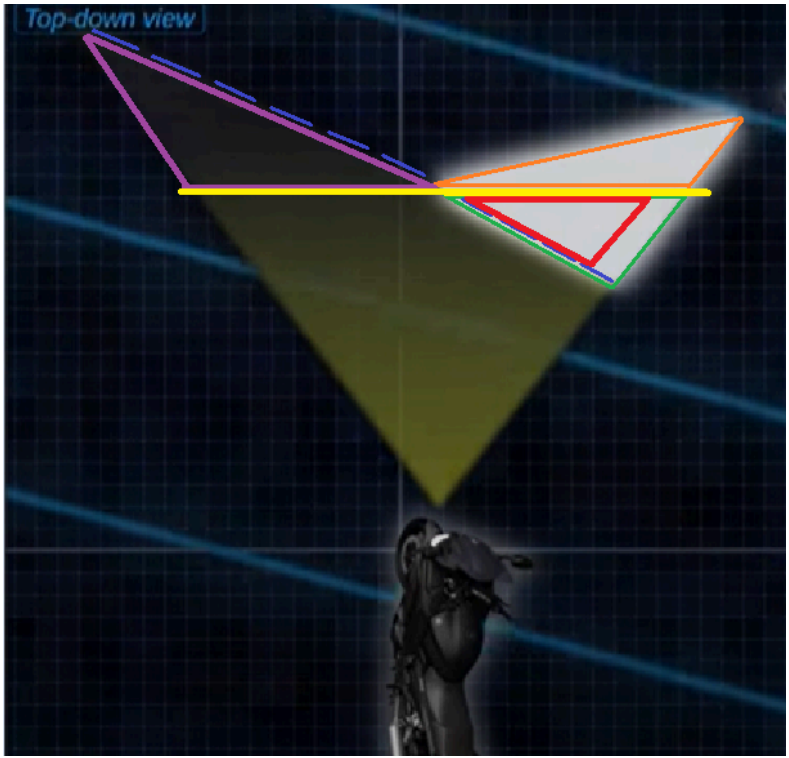
\includegraphics[width=0.75\linewidth]{Grafik/Cornering_Analysis_2.png}
    \caption{Lighting pattern changes with leaning at cornering}
    \label{cornering}
\end{figure}
\begin{itemize}
    \item \textbf{Yellow Line:} Horizontal line is the standard cut-off line when the motorcycle is level, which represents the transition between the high and low beam illumination zones
    \item \textbf{Blue Dashed Line:} Represents the low beam's horizontal alignment as the
    vehicle tilts, showing the change in the illumination pattern on the road. The
    area below this line is illuminated by the low beam, while the space above is
    illuminated by the high beam
    \item \textbf{Green Edged Triangle:} Represent the road section non-illuminated by low
    beam due to the vehicle's lean, requiring illumination for enhanced cornering
    visibility
    \item \textbf{Red Edged Triangle:} Represents the area illuminated by the pixel matrix high
    beam, limited compared to green triangle due to its matrix high beam’s narrower
    horizontal angle of illumination
    \item \textbf{Purple Edged Triangle:} Represents the area that must not be intensely
    illuminated to avoid causing glare, remaining non-adjustable due to the
    limitations of standard non-matrix low beams.
    \item \textbf{Orange Edged Triangle:} Represents the area that necessitates the application
    of an illumination gradient, guaranteeing a smooth fade-out from the light
    source to provide optimal visual comfort.
\end{itemize}

The principle of cornering compensation is designed to improve illumination on the side where the motorcycle is cornering. This means that as the motorcycle leans into a turn, the area of the apex, which typically suffers from poor lighting, receives enhanced illumination. This area is within the capabilities of the HD matrix's illumination range. The system's algorithm then activates specific pixels to project a triangular shaped light, effectively compensating for the lack of visibility in that area.  In the conclusion chapter effectiveness of the cornering compensation will be determined by error calculation method explain the \ref{method_error} ilumination coverage subchapter.

\subsection{Pitch Compensation Analysis}
Pitch compensation functionality of the motorcycle's headlight system is designed to address the change in the headlight beam's cut-off line that occurs when the motorcycle's nose dives during braking. The figure below offers a visual guide to how the lighting patterns change with braking at different pitch values. These changes are detailed in the bullet points that follow:
\begin{figure}[h!]
    \centering
    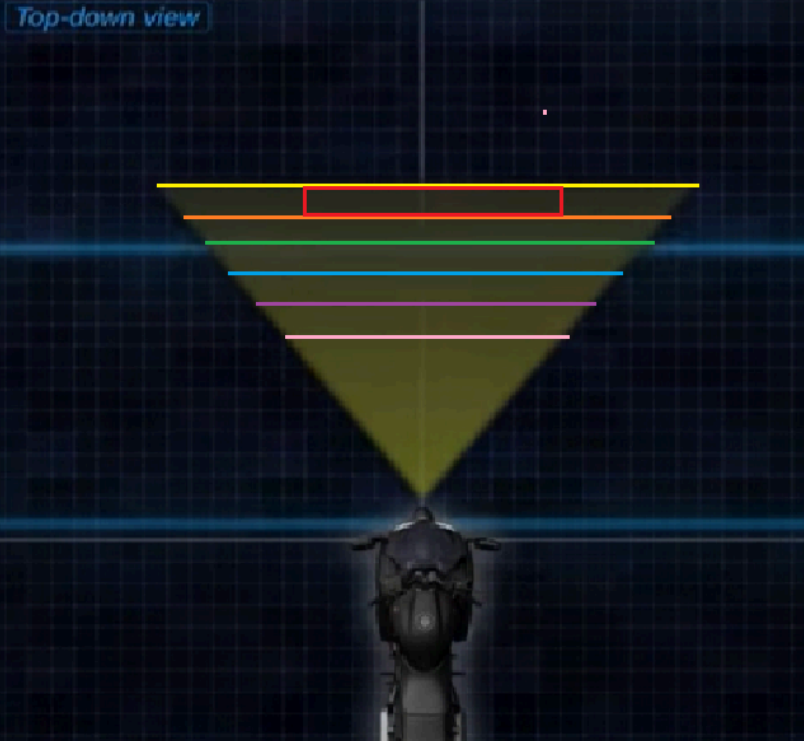
\includegraphics[width=0.75\linewidth]{Grafik/Pitch_Analysis_.png}
    \caption{Lighting pattern adjustments with braking at various pitch values}
    \label{pitch}
\end{figure}

\begin{itemize}
\item \textbf{0° Pitch - Baseline Illumination:} This is the standard cut-off line, represented
by the “yellow line” when the motorcycle is level, representing the transition
between the high and low beam illumination zones
\item \textbf{1° Pitch - Baseline Illumination:} Results in the cut-off line moving downward, a consequence of the
vehicle's nose dipping during braking, leading to a reduction in forward
illumination. The shifted cut-off line represented by the "orange line". The
red-edged rectangle illustrates the activation of a segment of the HD Matrix high
beam to counteract the minor downward displacement of the cut-off line caused
by the 1° pitch.
\item \textbf{Increased Pitch Angles:} As pitch angles increase, indicated by the green, blue, purple, and pink lines for 2°, 3°, 4°, and 5° pitches respectively, there's a corresponding downward shift in the cut-off line. This marks the transition from the upper boundary of the low beam to the lower edge of the high beam.
\end{itemize}

Consequently, pixel headlight system dynamically adjusts its illumination pattern with each pitch increment, where the upper edge of the illuminated area, marked by a red edge, moves upward to extend the light projection up to a yellow line, serving as the adjusted cut-off line. It calculates and compensates for the degree of pitch by activating the necessary pixels to maintain consistent visibility, effectively countering the dynamic cut-off line's displacement in real-time and ensuring enhanced road illumination 

In the conclusion chapter effectiveness of the cornering compensation will be determined by error calculation method explain the \ref{method_error} ilumination coverage subchapter


\subsection{Object Masking Analysis}
\textit{Currently waiting for a night ride with pixel headlight to get reference images}
%ADB ?


%% Re-consider the following



%\section{Methodology}
% Understanding requirements
% Feasibility Assesment
% System Design
% SW Development
% Verification And Validation

\begin{comment}
1. Understand the Requirements
		a. Safety concepts
			i. Performance levels PL (HARA)
			ii. Safety integrity levels
		b. Identify safety functions
			i. Overload protection
			ii. Emergency stop
			iii. Anti-collision system
			iv. Secure communication protocol
2. Risk Assesment
		a. Determine PL for each safety function
3. Design the System
		a. Select Appropriate components
			i. Harware, sensor, actuators
		b. System Architecture
4. Develop Safety-Related SW
		a. Adhere Guidelines
		b. Implement Safety Mesaures
			i. Safe state control, watchdog, error-handling 
Verification and Validation
\end{comment}

